\subsection{Modultest database}
\label{ssec: Modultest database}
Der er som gruppe taget en beslutning om at hoste databasen lokalt i en docker container. Dette blev valgt på baggrund af en samtale med vejleder, hvor vi blandt andet, grundet sikkerhedsforanstaltning på au’s netværk og problemer med microsoft licenser, kunne løbe ind i nogle problemer.
Den lokale hosting medførte at vi kunne holde øje med databasens udformningen, samt den gemte data, gennem Microsoft azure datastudie.\\

For at teste DAL funktioner og dens forbindelse til databasen, oprettes først et DAL objekt med en context som indeholder en korrekt connectionstring.
\begin{figure}[H]
\centering
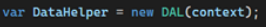
\includegraphics[width = 0.5\textwidth]{02-Body/Images/DAL-Database/DataHelper.png}
\caption{Oprettelse af DAL objekt med context indeholdende connectionstring}
\label{fig:Datahelper}
\end{figure}

Til test hvor der skal indsættes data i databasen oprettes der objekter af den korrekte type hvorefter DAL funktioner til indsættelse kaldes. Korrektheden af de indsatte data kan herefter tjekkes med datastudie.
Et eksempel på dette kan ses på \autoref{fig:SaveGame-test} herunder.
Her oprettes et GameDTO objekt, gamesave.\\
Gamesave opsættes til ”Gamer1”, med navnet ”My First Run”, hvorefter der tilføjes yderligere data. Det overskrevne save er ”NewGame1”, som her har id 1.

\begin{figure}[H]
\centering
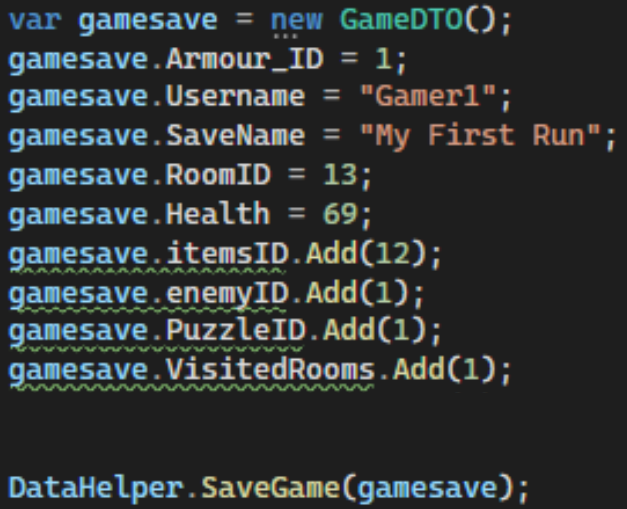
\includegraphics[width = 0.5\textwidth]{02-Body/Images/DAL-Database/NewSave-Test.png}
\caption{Kode til test af SaveGame, hvor der oprettes et nyt save som overskriver det gamle save med saveID 1}
\label{fig:SaveGame-test}
\end{figure}

På \autoref{fig:datastudie-før} herunder ses et screenshot fra datastudie hvor de 5 saves til ”Gamer1” kan ses.
Det noteres at alle saves er "tomme" og starter i rum 1.

\begin{figure}[H]
\centering
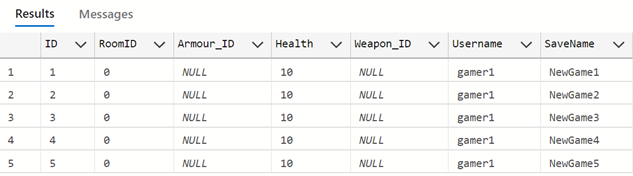
\includegraphics[width = \textwidth]{02-Body/Images/DAL-Database/DatastudieFørIndsættelse.png}
\caption{Screenshot fra datastudie hvor de 5 ens "tomme" saves kan ses}
\label{fig:datastudie-før}
\end{figure}

Herefter køres programmet fra \autoref{fig:SaveGame-test}, og vi kan nu se ændringerne i databasen.
Det noteres at SaveName og de andre attributter i \autoref{fig:datastudie-efter} nu er opdateret korrekt efter koden.

\begin{figure}[H]
\centering
\includegraphics[width = \textwidth]{02-Body/Images/DAL-Database/DataStudieEfterIndsættelse.png}
\caption{Sceenshot af datastudie efter overskrivning af save 1. Her er saveID 1 opdateret til nu at hedde "My First Run" og health og roomID er ændret korrekt, så det passer med det indsatte}
\label{fig:datastudie-efter}
\end{figure}

De øvrige tilhørende lister til det gemte save er også opdateret med korrekte værdie. Dette kan også ses på \autoref{fig:Datastudie-ekstra} herunder.

\begin{figure}[H]
\centering
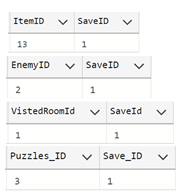
\includegraphics[width = 0.4\textwidth]{02-Body/Images/DAL-Database/Lister.png}
\caption{Sceenshot af datastudie efter overskrivning af save 1 med ekstra tabeller som referer til det rigtige saveID}
\label{fig:Datastudie-ekstra}
\end{figure}

Ved test af funktioner hvor der skal læses fra Db, kaldes DAL funktionen hvorefter den fundne information udskrives til konsolen ved hjælp af console writeline. Korrektheden af data i konsolen dobbelttjekkes med datastudie.
Et eksempel på dette ses på \autoref{fig:KodeTilLæsningAfSave} herunder.
Her henter vi det gemte save fra tidligere fra ”Gamer1” ved navn ”My First Run”, hvorefter data fra dette save udskrives i konsolen.

\begin{figure}[H]
\centering
\includegraphics[width = 0.5\textwidth]{02-Body/Images/DAL-Database/KodeTilLæsning.png}
\caption{Kode til test af GetSaveByID, hvor der hentes et save med saveID 1, hvoreft er det og tilhørende info udskrives på konsolen}
\label{fig:KodeTilLæsningAfSave}
\end{figure}

Når kodestykket fra \autoref{fig:KodeTilLæsningAfSave} ovenfor køres, får vi resultatet i konsol som set på \autoref{fig:Modulttest-consoleOutput} herunder.
Det noteres at det udskrevne data stemmeroverens med det indsatte data fra den tidligere funktionstest.

\begin{figure}[H]
\centering
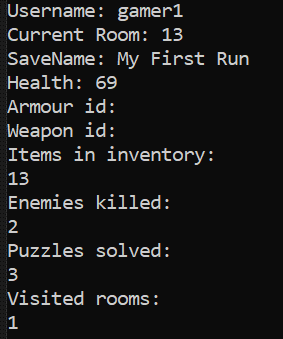
\includegraphics[width = 0.25\textwidth]{02-Body/Images/DAL-Database/ConsoleOutput.png}
\caption{Konsoleudskrift efter læsning af spil fra databasen, hvor det noteres at informationen stemmer overens med det indsatte i \autoref{fig:SaveGame-test}}
\label{fig:Modulttest-consoleOutput}
\end{figure}


I \autoref{table:Modulttest-DB-Tabel} herunder ses en tabel over udførte test, forventede resultater, den faktiske observering og vurderingen af observeringen.
Alle test er udført og vi observerer det forventede resultat. Vi vurderer derfor alle test som OK.

\begin{table}[H]
\caption{Tabel over modulttest af DAL forbindelse til databsen. Alle test observeringer stemmeroverens med forventningerne og markeres derfor OK }
\label{table:Modulttest-DB-Tabel}
\begin{tabular}{|p{0.75cm}|p{3.6cm}|p{3.5cm}|p{3.5cm}|p{1.9cm}|} \hline
\multicolumn{5}{|c|}{\textbf{DAL-Database Godkendelses Tabel}} \\ \hline
 \textbf{Test} & \textbf{Funktion} & \textbf{Forventet resultat} & \textbf{Observering} & \textbf{Vurdering} \textbf{(OK/Fail)}\\\hline
 1 & GetRoomDescription(id) & Her forventes det at funktionen henter beskrivelsen fra den valgte rumId. & Funktionen henterbeskrivelsen korrekt og vi kan udskrive denne på konsolen. & OK \\ \hline
 2 & GetAllSaves & Det forventes at alle spillets saves, med tilhørende info, hentes fra databasen & Alle saves hentes fra databasen og information om disse kan udskrives på konsolen. & OK \\ \hline
 3 & GetSaveById(id) & Det forventes at der hentes alle oplysninger om et enkelt save fra databasen med tilsvarende id, som den medsendte parameter & Det korrekte save samt tilhørende info hentes og kan udskrive til konsolen & OK \\ \hline
 4 & SaveGame(Game) & Det forventes at det valgte save med samme id som det nye, overskrives, og at tilhørende info opdateres & Det observeres at det gamle save med samme id, nu er ændret og har korrekte nye værdier & OK \\ \hline
\end{tabular}
\end{table}

\subsubsection{Diskussion af database modultest}

Den ovenstående modultest er generelt godkendet da alle funktioner opfører sig som forventet, i og med at der hentes og gemmes korrekt i databasen. Med alle funktioner testet og godkendt er DAL-database forbindelsen klar til at blive integreret med resten af systemet.
